\documentclass[11pt,letterpaper]{article}
\usepackage[margin=1in]{geometry}
\usepackage[T1]{fontenc}
\usepackage{lmodern,amsmath,amssymb,amsthm,booktabs,graphicx,longtable,pdflscape,needspace}
\usepackage{natbib}
\usepackage[hyphens]{url}
\usepackage[hidelinks]{hyperref}
\newtheorem{proposition}{Proposition}
\title{Which Uncertainty Is Worth Reducing?\\Technical Supplement}
\author{Anonymous Submission}
\date{}
\hypersetup{pdftitle={Which Uncertainty Is Worth Reducing? Technical Supplement},pdfauthor={}}
\begin{document}
\maketitle
\noindent This supplement documents assumptions, proofs, data construction, computational checks and all declared primary experiment settings. Public-data replay and conditional NHS illustrations do not constitute a field intervention.
\section{Exploratory Budget Extension}
After inspecting the primary replay results, we specified a separate budget extension to test whether the short-budget comparison persists when more reference measurements are affordable. The extension protocol was recorded before its own execution, but after the primary analysis; it is therefore exploratory. It does not replace the original grid. It fixes the unweighted tilt-0.50 replay, validation cost 5, all previous-year calibration, budgets 48, 144, 480 and 1,440, and 500 repetitions with a new seed. The same unit-channel packet bank is reused across the four budgets and all five policies. All outcomes from this grid are reported, including those unfavourable to two-channel KG.

\begin{table}[htbp]
\centering\small\begin{tabular}{lrrrrr}
\toprule
Budget & Ord. KG & Two KG & Balanced & Val. only & Uniform \\
\midrule
48 & 0.1794 & 0.1957 & 0.1972 & 0.1986 & 0.1988 \\
144 & 0.1593 & 0.1867 & 0.1897 & 0.1882 & 0.1815 \\
480 & 0.1367 & 0.1500 & 0.1800 & 0.1635 & 0.1605 \\
1440 & 0.1242 & 0.0907 & 0.1499 & 0.1229 & 0.1380 \\
\bottomrule
\end{tabular}

\caption{Exploratory budget extension: mean severity regret, 500 paired repetitions at each budget. This is a separate run from the 1,000-repetition primary grid. The complete CSV includes actual spending and paired Monte Carlo intervals.}
\end{table}

Two-channel KG remains worse than ordinary KG at budgets 48, 144 and 480. At budget 1,440, the comparison reverses: regret is 0.09070 versus 0.12422, a paired difference of $-0.03352$ with 95\% Monte Carlo interval [$-0.03793$,$-0.02910$]. This is evidence of a budget-dependent comparison within the specified replay, not a measured NHS cost threshold. At budgets 480 and 1,440, two-channel KG spends all additional resources on validation. The improvement must not be described as successful balancing of two channels. At 1,440, uniform validation also uses only validation, spends the same budget, and has regret 0.12288; the comparison with KG concerns which units receive those reference packets. The budget is 30 ordinary-packet cost equivalents per area, or 288 validation packets in total at cost 5, on top of the shared initial observations. A real price per completed packet is not inferred.

\begin{figure}[htbp]
\centering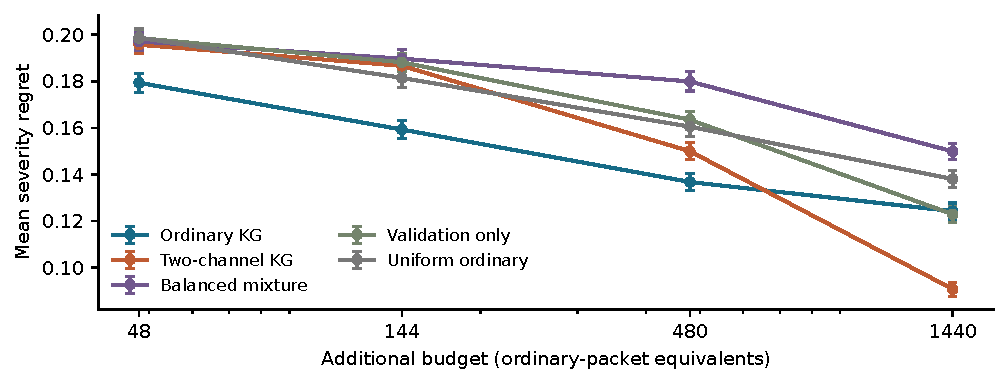
\includegraphics[width=\textwidth]{figures/budget_extension.pdf}
\caption{Exploratory budget sensitivity on one controlled replay mechanism. Error bars are 95\% Monte Carlo intervals. All four budgets were specified before running this extension. Ordinary-only policies cannot access validation; the balanced mixture and validation-only policy provide comparisons with that access.}
\end{figure}

\section{Estimation, Cost and Misspecification Diagnostics}
The MSE/regret comparison makes the target dependence of acquisition tangible. MSE averages squared level errors across every unit; severity regret evaluates only the selected set relative to the oracle with the same quota. A small reduction in aggregate MSE can coexist with a less accurate ordering around the selection boundary. The replay comparisons below are descriptive effects of full policies. They do not isolate how much of the difference is due to Gaussian approximation, prior calibration, per-packet noise, cost or myopic action choice.

\begin{table}[htbp]
\centering\small\begin{tabular}{lrrrrr}
\toprule
Scenario & Ord. loss & Two loss & Ord. MSE & Two MSE & Val. cost \\
\midrule
Uniform & 0.1124 & 0.1124 & 0.01802 & 0.01802 & 0.0\% \\
Tilt 0.25 & 0.1570 & 0.1755 & 0.02116 & 0.02092 & 90.2\% \\
Tilt 0.50 & 0.1615 & 0.1857 & 0.02183 & 0.02129 & 97.2\% \\
Weighted tilt & 0.1773 & 0.1959 & 0.02250 & 0.02194 & 97.2\% \\
Biased validation & 0.1612 & 0.2226 & 0.02182 & 0.02308 & 97.2\% \\
\bottomrule
\end{tabular}

\caption{Primary replay at budget 144 and validation cost 5. ``Ord.'' and ``Two'' refer to ordinary-only and two-channel KG with matched bias-aware inference. Validation cost is the fraction of the two-channel policy's budget spent on that channel. Target MSE and selection loss are distinct.}
\end{table}

\begin{figure}[htbp]
\centering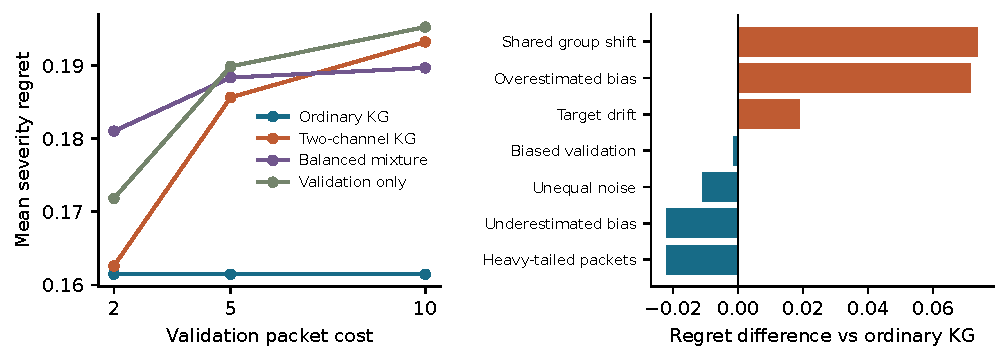
\includegraphics[width=\textwidth]{figures/cost_and_stress.pdf}
\caption{Left: validation-cost sensitivity on tilt-0.50 replay at budget 144. Right: synthetic stress-world regret differences at budget 120 and cost 5; positive values favour ordinary KG. All stress results remain in the numerical release, including small or adverse comparisons.}
\end{figure}

\section{Research Transparency}
This study uses public aggregate NHS data and public-use BRFSS records. It conducts no new recruitment, intervention or private-data linkage. The computational benchmark does not attribute individuals' mental health to their jobs and does not diagnose a clinical condition. Source: CDC BRFSS. This independent research and its conclusions are not endorsed by CDC, HHS, the United States Government or NHS organisations. Existing source terms continue to govern original materials; a licence for newly authored code does not relicense agency materials.

AI assistance was used extensively for literature discovery, mathematical derivation, code generation, numerical auditing, analysis and manuscript preparation. Automated checks and independent implementations are documented; they do not replace the named author's responsibility for reviewing the manuscript, verifying references, understanding the analysis and approving any submission. No external stakeholder co-design, ethics approval, funding award or deployment is claimed. No real institutional allocation has been made from the research. Authorship and any necessary institutional declarations must accurately reflect the actual work and affiliation when submitted.

The source package contains runnable experiment scripts, derived public-data frames, complete summary CSVs, a results workbook, acquisition/source manifests, numerical-verification scripts, local analysis protocols and source snapshots for the primary runs. Detailed simulation metrics can be regenerated with the stored seeds. The separate exploratory extension also retains replication-level arrays. Working-directory paths and personal identifiers are excluded from the anonymous PDF text. Public-data access, re-download and source validation depend on continued availability of the cited official releases; included derived-data reproduction does not require private credentials or a GPU.

\appendix
\section{Notation and Complete Reference-Model Results}
The propositions below restate the model self-containedly. To distinguish local notation from channel cost, the off-diagonal covariance is denoted $c_i$ in these propositions (the main paper calls it $u_i$). Channel cost is written explicitly as $\operatorname{cost}_{id}$. The results concern the declared independent-unit Gaussian model with fixed hyperparameters. They do not infer real survey bias from aggregate scores.
% Integration fragment. Requires amsmath, amssymb, amsthm, natbib;
% define a proposition environment in the main preamble.
% Full proofs are in theory_proofs.tex, to be input after \appendix.
% Root may shorten or adapt notation; no empirical conclusions are asserted here.

\section{Decision value of another measurement}
\label{sec:information_theory}
Let $\mathcal S=\{S:|S\cap g|=k_g\text{ for every group }g\}$,
$K=\sum_g k_g>0$, and let lower $\theta_i$ mean greater need. We use
\begin{equation}
 L(S,\theta)=\frac{1}{K}\left\{\sum_{i\in S}\theta_i-
          \min_{A\in\mathcal S}\sum_{i\in A}\theta_i\right\}.
 \label{eq:aisi_loss}
\end{equation}
Thus review slots have equal weight across all selected units; this is not
equal weighting of group-specific average losses. The Bayes decision selects
the $k_g$ smallest posterior target means within each group. Linearity of
expectation suffices for this decision, even with dependent targets.
Neither this loss nor its minimizer is a probability-of-exact-set-recovery
objective. Fixed-budget subset selection and boundary-directed acquisition
have substantial prior art \citep{chen2008subset,kalyanakrishnan2012pac,chen2014combinatorial}.

For the acquisition calculation, assume independent unit states, fixed
hyperparameters, and a Gaussian posterior
$(\theta_i,b_i)\mid D\sim N((m_i,a_i)^{\mathsf T},P_i)$, where
$P_i=\left(\begin{smallmatrix}v_i&c_i\\c_i&q_i\end{smallmatrix}\right)$.
An ordinary packet measures $\theta_i+b_i$; an ideal validation packet
measures $\theta_i$. Their loadings are $h_R=(1,1)^{\mathsf T}$ and
$h_A=(1,0)^{\mathsf T}$. A packet has conditionally independent Gaussian
noise variance $r_{id}>0$. Its posterior-mean innovation has standard deviation
\begin{equation}
 s_{id}=\frac{|(P_i h_d)_1|}{\sqrt{h_d^{\mathsf T}P_i h_d+r_{id}}}.
 \label{eq:aisi_innovation}
\end{equation}
For $a$ independent respondent draws with individual noise variance $r$,
the packet mean has variance $r/a$; a persistent offset does not shrink this way.
Conditional unbiasedness of the validation channel is a reference-model
assumption, not a property inferred from the NHS data.

\begin{proposition}[One-step severity value]
\label{prop:aisi_kg}
For an action affecting only unit $i$ in a group with $0<k_g<|g|$, let
$t_i$ be the $k_g$th smallest posterior mean among the other units in that
group and set $\Delta_i=|m_i-t_i|$. Its expected reduction in posterior
Bayes risk is
\begin{equation}
 \operatorname{KG}_{id}=\frac{1}{K}
 \left\{s_{id}\varphi(\Delta_i/s_{id})-
         \Delta_i\Phi(-\Delta_i/s_{id})\right\},
 \label{eq:aisi_kg}
\end{equation}
with value zero at $s_{id}=0$. Groups selecting none or all of their units
have zero local acquisition value. For finite gaps and positive $s$, the
value strictly increases with $s$ and decreases with the gap.
\end{proposition}

This is a closed-form specialization of Gaussian knowledge gradient
\citep{frazier2008kg,frazier2009correlated}, closely related to
multi-information-source optimization \citep{poloczek2017miso}; it is not
a new subset-selection algorithm. Our policy compares affordable actions
by $\operatorname{KG}_{id}/\operatorname{cost}_{id}$. The common $1/K$
factor can be omitted when choosing the action. This myopic cost ratio is
not globally optimal for a fixed multistep budget; Appendix~\ref{app:aisi_theory}
gives a counterexample, consistent with known nonconcavity of information
value \citep{frazier2010paradoxes}. If an observation updates several units,
Equation~\eqref{eq:aisi_kg} must be replaced by the joint decision value.

\begin{proposition}[Limits of repeated ordinary measurement]
\label{prop:aisi_floor}
Suppose $\theta\sim N(\mu,\tau^2)$ and $b\sim N(0,\beta^2)$ are independent,
with $\tau,\beta>0$, and $Y_j=\theta+b+\epsilon_j$ has independent
$\epsilon_j\sim N(0,r)$. Then
\begin{equation}
 \operatorname{Var}(\theta\mid Y_{1:n})
 =\tau^2-\frac{\tau^4}{\tau^2+\beta^2+r/n}
 \longrightarrow \frac{\tau^2\beta^2}{\tau^2+\beta^2}.
 \label{eq:aisi_level_floor}
\end{equation}
For two independent units with this common prior and one review slot, even
exactly observing both $\theta_i+b_i$ leaves Bayes severity regret
\begin{equation}
 R_\infty=\frac{\tau}{\sqrt{\pi}}
          \left(1-\frac{\tau}{\sqrt{\tau^2+\beta^2}}\right)>0.
 \label{eq:aisi_selection_floor}
\end{equation}
This is a lower bound for every policy restricted to noisy ordinary
measurements under that prior, including adaptive policies.
\end{proposition}

The explicit selection-risk expression concerns independent unit-specific
offsets. Partial identification despite unlimited samples is a broader,
established phenomenon \citep{altschuler2019contaminated}; the next result
shows why level uncertainty alone does not establish selection harm.

\begin{proposition}[Shared group shifts do not change this loss]
\label{prop:aisi_shared}
For arbitrary constants $u_g$, define $\theta'_i=\theta_i+u_g$ for $i\in g$.
For every feasible $S$, $L(S,\theta')=L(S,\theta)$, and the collection of
optimal feasible sets is unchanged. Consequently, if the only persistent
ordinary-channel offset is common within each group, exact ordinary means
identify an optimal within-group selection even when target levels remain
unidentified.
\end{proposition}

Thus a useful measurement reduces uncertainty about relevant differences,
not necessarily about absolute levels. A policy that models common offsets
as independent unit offsets can value validation for distinctions that are
irrelevant to fixed within-group slots.

\begin{proposition}[When a second channel resolves uncertainty]
\label{prop:aisi_channel}
In the independent-unit reference model, ideal validation has greater
one-step value than an ordinary packet at the same unit and equal cost
if and only if
\begin{equation}
 \frac{v_i^2}{v_i+r_{iA}}>
 \frac{(v_i+c_i)^2}{v_i+q_i+2c_i+r_{iR}},
 \label{eq:aisi_switch}
\end{equation}
provided the group has a nontrivial quota. If $c_i=0$ and $v_i>0$, this
reduces to $r_{iA}<q_i+r_{iR}$. If validation instead measures
$\theta+d$ with a second persistent offset, independent priors with positive
variances $\tau^2,\beta^2,\delta^2$ imply
\begin{equation}
 \operatorname{Var}(\theta\mid\theta+b,\theta+d)
  =(\tau^{-2}+\beta^{-2}+\delta^{-2})^{-1}>0.
 \label{eq:aisi_two_biased}
\end{equation}
Independence between channel offsets therefore does not suffice to make
validation unbiased for an individual unit.
\end{proposition}

For unequal costs, the comparison uses the full cost-normalized expression
in Equation~\eqref{eq:aisi_kg}, not merely variance reduction per cost.
Cheap biased sources versus expensive reference sources are already central
to multi-fidelity identification \citep{poiani2024optimal} and selective
proxy auditing \citep{ao2026judges}. These propositions characterize which
parts of that information problem matter for this decision; they do not
identify unknown survey bias or provide guarantees under misspecified
channel models.

% Input in supplementary material, after \appendix. Requires theory_sections.tex.
\section{Proofs and an allocation counterexample}
\label{app:aisi_theory}

\paragraph{Bayes decision and Gaussian update.}
Conditional on $D$, the oracle term in Equation~\eqref{eq:aisi_loss} is
independent of the chosen set. Thus minimizing expected loss is equivalent
to minimizing $\sum_{i\in S}m_i$ subject to the fixed quotas. A deterministic
index rule may resolve equal means without changing the objective.
For a Gaussian linear observation $W=h^{\mathsf T}(\theta,b)+\epsilon$,
write $V=h^{\mathsf T}Ph+r>0$. Conditioning yields
\[
 P^+=P-Phh^{\mathsf T}P/V,\qquad
 m^+=m+(Ph)_1\{W-h^{\mathsf T}(m,a)\}/V.
\]
The predictive residual is $N(0,V)$, which proves
Equation~\eqref{eq:aisi_innovation}. This calculation conditions on fixed
hyperparameters; learning a shared hyperparameter from the new observation
can also update other units and invalidate the one-coordinate simplification.

\begin{proof}[Proof of Proposition~\ref{prop:aisi_kg}]
Order the other units' means as $a_{(1)}\le\cdots\le a_{(|g|-1)}$.
With $t_i=a_{(k_g)}$, the optimal posterior-mean sum in this group equals
$\sum_{j<k_g}a_{(j)}+\min(m_i,t_i)$. After the observation, replace
$m_i$ by $m_i+sZ$, where $Z\sim N(0,1)$; all other group contributions
are unchanged. The tower property cancels the expected oracle-loss term
from the before/after Bayes risk. Therefore the value is
\[
 K^{-1}\{\min(m_i,t_i)-\mathbb E\min(m_i+sZ,t_i)\}
 =K^{-1}\mathbb E(sZ-|m_i-t_i|)_+.
\]
Integrating the Gaussian tail gives Equation~\eqref{eq:aisi_kg}.
For $s>0$ and $\Delta\ge0$, differentiation gives
$\partial(K\operatorname{KG})/\partial s=\varphi(\Delta/s)>0$ and
$\partial(K\operatorname{KG})/\partial\Delta=-\Phi(-\Delta/s)<0$.
At $s=0$, the mean does not change and the value is zero. For a quota
of zero or the entire group, the feasible choice in that group is fixed;
the tower property gives zero expected improvement. Equal means cause no
problem because the optimum sum, rather than a discontinuous membership
indicator, is the value function.
\end{proof}

\begin{proof}[Proof of Proposition~\ref{prop:aisi_floor}]
The sample mean is sufficient and has variance
$\tau^2+\beta^2+r/n$, with covariance $\tau^2$ with $\theta$.
Gaussian conditioning proves Equation~\eqref{eq:aisi_level_floor}.
For two units, set $T_i=\theta_i+b_i$. Their conditional means
$m_i=\mu+\lambda(T_i-\mu)$, with
$\lambda=\tau^2/(\tau^2+\beta^2)$, are independent normals with
standard deviation $\tau^2/\sqrt{\tau^2+\beta^2}$. The minimum of two
independent normals of common mean $\mu$ and standard deviation $s$
has expectation $\mu-s/\sqrt{\pi}$. Hence
\[
 \mathbb E\min(m_1,m_2)-\mathbb E\min(\theta_1,\theta_2)
 =\frac{\tau}{\sqrt\pi}
   -\frac{\tau^2}{\sqrt{\pi(\tau^2+\beta^2)}},
\]
which is Equation~\eqref{eq:aisi_selection_floor}. Any adaptive sequence
of ordinary observations can be simulated from exact $(T_1,T_2)$ and
independent observation and policy randomness. Exact $T$ therefore
contains at least as much decision-relevant information as that sequence;
its optimal Bayes risk is a lower bound for all such policies.
\end{proof}

\paragraph{A current-posterior version of the variance floor.}
For arbitrary positive-semidefinite $P$ with entries $(v,c,q)$, exact
knowledge of $T=\theta+b$ leaves
$v-(v+c)^2/(v+q+2c)$ when $\operatorname{Var}(T)>0$.
If $\operatorname{Var}(T)=0$, $T$ is already known and its acquisition
does not change $v$; positive semidefiniteness implies $v+c=0$.
After learning $T$ exactly, $\operatorname{Cov}(\theta,T\mid T)=0$,
so further ordinary sampling has zero target-mean innovation. Under
independent units, positive remaining $v$, a nontrivial quota, and finite
noise, ideal validation still has strictly positive one-step value.
Affordability and the amount of remaining budget are separate constraints.

\begin{proof}[Proof of Proposition~\ref{prop:aisi_shared}]
Every feasible set has the same additional sum $\sum_g k_g u_g$ under
the transformation. It appears both in the selected-set sum and the
minimized oracle sum, so it cancels. All comparisons among feasible sums
are also unchanged. If ordinary means equal $\theta_i+b_g$, this same
argument applies with $u_g=b_g$ to recover the optimal feasible sets.
\end{proof}

\paragraph{Why marginal uncertainty can be irrelevant.}
For two units with $\theta_1=\theta_2=Z$, $Z\sim N(0,1)$, and one slot,
the selection regret is always zero. An exact observation of either unit
updates both posterior means to $Z$, so the true joint information value
is zero. Updating only one coordinate incorrectly would give
$\varphi(0)=1/\sqrt{2\pi}$. This shows why the independence/one-coordinate
assumption of Proposition~\ref{prop:aisi_kg} matters when offsets or targets
have shared structure.

\begin{proof}[Proof of Proposition~\ref{prop:aisi_channel}]
At the same unit the gap is the same for both actions, and
Proposition~\ref{prop:aisi_kg} is strictly increasing in $s$.
Substituting $h_A$ and $h_R$ into Equation~\eqref{eq:aisi_innovation}
and comparing squared innovations gives Equation~\eqref{eq:aisi_switch}.
For $c=0$ and $v>0$, the equal numerators $v^2$ cancel.
For the final statement, conditional on $\theta$, exact $T=\theta+b$
and $U=\theta+d$ have independent likelihoods with variances $\beta^2$
and $\delta^2$. Adding their precisions to the prior precision proves
Equation~\eqref{eq:aisi_two_biased}. Repeated independent observation
noise can reveal $T$ and $U$, but it does not remove their persistent
offsets. If both channels instead share the same offset, their exact
values supply only one such equation.
\end{proof}

\paragraph{A fixed-budget counterexample to the cost ratio.}
There is one known alternative of value zero and one target
$\theta\sim N(0,1)$, with one slot and budget two. A cheap direct
measurement of $\theta$ has noise variance one and cost one. A more
accurate direct measurement has noise variance $0.1$ and cost two.
Both have zero initial gap. Their initial knowledge gradients are
$1/\sqrt{4\pi}=0.282095$ and
$1/\sqrt{2.2\pi}=0.380377$, respectively. Their cost ratios therefore
favor the cheap action: $0.282095>0.190188$. Only another cheap action
is affordable afterward. The two cheap measurements produce posterior
mean variance $2/3$, hence total expected improvement
$\sqrt{2/3}/\sqrt{2\pi}=0.325735$. Spending the budget on the more
accurate action yields $0.380377$, a larger value. The policy can fail
even with correct Gaussian beliefs and conditionally unbiased channels;
one-step value per cost is not the multistep budget objective.


\section{Algorithms and Exact Computation}
\subsection{Policy state and update}
Each replication starts with a two-coordinate state per unit. Its state stores target mean, offset mean, target variance, offset variance, their covariance, and ordinary/validation draw counts. For each unit $i$ and affordable channel $d$, compute the relevant other-unit quota boundary $t_i$, the innovation SD and Equation~\eqref{eq:aisi_kg}. Choose the action with maximum gain per cost, read the next unused entry in that unit-channel observation stream, apply Gaussian conditioning, and deduct the channel cost. Ties use deterministic flattened unit/channel order for KG-based rules. Recompute boundaries after every observation. The final review set consists of the smallest posterior means within each group, with stable index ties.

One update has constant cost per affected unit. Computing all boundaries by sorting costs $O(M\log M)$ per replication in this implementation; evaluating $2M$ action values is linear. The implementation is vectorised over independent replications. It does not claim an optimal computational complexity or a new data structure. Finite-precision normal-tail calculations are clamped to nonnegative values to avoid tiny cancellation artefacts. A budget is integer-valued and checked at every step. Validation-only policies may leave a remainder smaller than the validation cost. Comparisons report both available budget and actual spending.

\subsection{Ten policy definitions}
\begin{enumerate}
\item Uniform ordinary: choose a unit uniformly and acquire an ordinary packet, retaining the common bias-aware posterior.
\item Uniform, bias blind: the same action rule with assumed bias mean and variance zero.
\item Maximum variance: acquire an ordinary packet at the unit with largest target posterior variance.
\item Boundary heuristic: acquire ordinary data at the largest $2\sqrt{v_i}-|m_i-t_i|$. This fixed-budget heuristic is not the LUCB algorithm.
\item Ordinary KG: maximise one-step severity gain using only ordinary packets.
\item Bias-blind KG: ordinary KG with zero assumed offset.
\item Equal-action mixture: sample uniformly over affordable unit-channel pairs. Equal action probability does not mean equal expenditure.
\item Balanced mixture: before affordability effects, choose validation with probability $1/(1+c_A)$ and a uniform unit; otherwise ordinary. If a requested validation packet is unaffordable, use an ordinary packet. This balances expected expenditure before terminal effects.
\item Validation only: choose a uniform unit and use only validation after the common initial ordinary phase. Stop when no validation packet is affordable.
\item Two-channel KG: maximise one-step severity gain per cost over both affordable channels, using the same posterior update as the bias-aware baselines.
\end{enumerate}
The full-code release also contains a dormant terminal-rule variant used for implementation exploration; no reported experiment uses it. Shared inference distinguishes action selection from the benefits of assuming a bias model. Common channel access distinguishes two-channel acquisition efficiency from the value of access to a different measurement source.

\subsection{Pairing, estimation and stopping}
Each world or replay scenario generates a packet bank indexed by replication, unit, channel and within-channel packet count. Policies observing the same count for the same unit-channel pair see the same packet, regardless of their elapsed action number. Latent worlds and banks are shared across cost and budget settings within a primary scenario. Independent policies may take different numbers of packets, but do not overwrite or consume another policy's bank. Randomised baselines have explicit seeds.

For $R$ independent replications and a metric $z_r$, the stored MCSE is $s(z)/\sqrt R$ and the displayed interval is $\bar z\pm1.96\,\mathrm{MCSE}$. For two policies, compute the differences $z_r^{(1)}-z_r^{(0)}$ first and apply the same calculation; do not combine their marginal standard errors as if they were independent. Primary CSVs store paired regret and overlap comparisons with ordinary KG and bias-aware uniform ordinary. The exploratory extension retains replication-level arrays to verify these computations. No cross-scenario pooled significance test is reported, and simultaneous coverage over the full grid is not claimed.

In finite-file replay, a \emph{fixed-length primitive packet mean} from iid uniform record draws is unbiased for its declared finite-frame mean. Under weight-proportional sampling it is unbiased for the constructed weight-proportional distribution. This statement does not make the final posterior estimate, or a unit's empirical mean after outcome-adaptive sampling, unbiased. Counts depend on observed outcomes. Interval coverage is calculated against each fixed-frame target across replay repetitions; it does not establish design-based population coverage.

\section{Synthetic Worlds in Full}
Targets are independent $N(5,0.35^2)$ for 40 units, arranged in four groups of ten with quota two. In the base worlds, an offset $b_i\sim N(0,\beta^2)$ persists across initial and subsequent ordinary packets. Validation has fresh noise and no persistent offset. Initial sample size and additional packet size both equal 20. Conditional packet-noise SD is $2.5/\sqrt{20}$. Budgets are 40 and 120, validation costs 2, 5 and 10, and ordinary cost one. Four bias scales and six cost/budget pairs yield 24 settings and 240 policy rows. Each of the four worlds has 2,000 independent replications; the 24 settings are not 48,000 independent latent panels.

Seven stress worlds add 70 policy rows, each with 2,000 independent replications, budget 120 and validation cost 5. Underestimated bias uses true SD 0.70 and assumed SD 0.15; overestimated bias uses true SD zero and assumed SD 0.70. The validation-bias world adds an independent persistent validation offset with SD 0.35 while the update treats validation as unbiased. The heavy-tail world replaces Gaussian packet noise with Student-$t_3$ noise scaled to the same packet variance. It draws heavy-tailed \emph{packet} means directly; a packet is not implemented as an average of 20 individual heavy-tailed observations. Unequal noise multiplies each unit's noise SD by a lognormal factor with log SD 0.4 while inference keeps the common SD. Target drift adds independent $N(0,0.35^2)$ changes after initial observations; all later observations measure the changed target while inference assumes a static state. Shared-group bias uses a single SD-0.70 offset per group, but inference treats offsets as independent. Unless specified otherwise, true and assumed bias SDs are 0.35.

All seven stresses are deliberately misspecified relative to the exact propositions. The purpose is to locate failures, not to claim robustness from passing a chosen subset. Uniform/blind baselines use the same observation law as other policies within a world. Unit-mean target MSE and interval coverage concern the post-drift target where applicable. Unbounded Gaussian targets are a controlled mathematical world, not a generative model claiming that NHS scores can lie outside their scale.

\section{Public Microdata Construction and Temporal Separation}
\subsection{Source and cleaning}
The downloaded 2023 BRFSS ASCII file contains 433,323 records; the 2024 file contains 457,670. Official SAS import programs and variable-layout documentation determine required ASCII offsets. Reading streams from ZIP members avoids expanding gigabyte-size text files. The required variables are state, core mental-health days, employment, final combined survey weight, stratum, PSU and the supplied mental-health category used for validation. Core outcome codes 1--30 and 88 are valid; 77, 99 and blanks are excluded. Employment codes 1 and 2 denote employed for wages and self-employed. The score is a transparent rescaling, not a newly validated wellbeing questionnaire or a measure of job-caused distress.

\begin{table}[htbp]
\centering
\begin{tabular}{lrr}\toprule
Cleaning stage & 2023 & 2024\\\midrule
Complete public file & 433,323 & 457,670\\
Employed/self-employed before outcome filtering & 215,794 & 225,524\\
Employed with valid outcome, all areas & 212,989 & 222,734\\
Common-state/DC complete-outcome frame & 206,098 & 214,151\\
Number of common areas & 48 & 48\\
Minimum records per included area & 1,247 & 1,232\\
Maximum records per included area & 13,474 & 22,708\\\bottomrule
\end{tabular}
\caption{Executed BRFSS cohort construction. The cross-year intersection excludes territories, Kentucky and Pennsylvania (absent from 2023), and Tennessee (absent from 2024). Annual files are independent cross-sections, not a person panel.}
\end{table}

All 420,249 cleaned primary records were independently compared with the original ASCII slices. All 457,670 original 2024 records were also checked against the official SAS-transport file: categorical/design fields agree, and the maximum absolute weight discrepancy is $4.997\times10^{-5}$ from the ASCII representation's decimal precision. Four employed Illinois records have a core mental-health response inconsistent with the supplied categorical derivative. The same discrepancy exists in both original formats. We keep the core responses, record the discrepancy and do not selectively correct or exclude those records. This check demonstrates why matching aggregate codebook frequencies alone is insufficient.

The actual compressed ASCII sizes were 60,057,185 and 53,411,907 bytes. The acquired 2024 text has 2,061-character records, despite a stale longer-file description on the annual webpage. Source offsets are verified against the actual import programs and layout entries; page descriptions do not override measured files. Retrieval timestamps, resolved URLs, byte counts, SHA-256 hashes and ZIP member CRCs identify the downloaded releases. These are locally computed identity checks, not publisher-supplied hashes or claims of access to the first published vintage.

\subsection{Targets and the sampling mechanism}
For area $i$ and year $y$, let $p_{iy}(x)$ be the empirical probability of score $x$ among complete employed records. The primary target is $\theta_{i,2024}=\sum_xp_{i,2024}(x)x$. All 2024 means are reserved for final evaluation. A fixed 2023 common target prior uses $\mu=8.55693$ and $\tau=0.13882$, calculated from its 48 area means. The 2023 within-area variance supplies packet-noise calibration. No held-out 2024 full-frame moment is given to the action selector.

For a random sign $s_i\in\{-1,+1\}$ fixed throughout a replication, the ordinary sampler uses
\[
 p_{i,2024}^{(s_i)}(x)=\frac{p_{i,2024}(x)\exp\{s_i\kappa(x-\mu_{i,2023})/\sigma_{i,2023}\}}
 {\sum_zp_{i,2024}(z)\exp\{s_i\kappa(z-\mu_{i,2023})/\sigma_{i,2023}\}}.
\]
Centering cancels from the normalisation; the scale remains frozen to 2023. The same plus/minus construction on 2023 gives two hypothetical mean offsets. Their midpoint is the assumed bias mean; their population SD is the assumed bias SD. The average of the two within-law variances supplies ordinary noise. This centre is not generally zero because the outcome distribution is asymmetric. For $\kappa=0.25$ and 0.50, the average calibrated bias SDs are approximately 0.6865 and 1.4952, respectively. These are deliberately strong controlled tilts relative to the between-area spread, not plausible-bias estimates derived from actual recruitment validation.

Validation draws uniformly from the hidden empirical distribution except in its separate failure scenario. There it has an independent persistent sign and tilt 0.25, yet the update continues to assume an unbiased channel. The exact two-sign mechanism is not fitted as a discrete posterior; the policy deliberately uses the same moment-matched Gaussian approximation. Its calibration is favourable because it knows a hypothetical sampling-law family, but it is not an oracle using realised 2024 offsets or reference means.

Weighted sensitivity replaces $p_{iy}$ by the empirical probability proportional to each record's final survey weight. Its target is $\sum_jw_jx_j/\sum_jw_j$ in the retained finite file. The common 2023 prior has $\mu=8.41342$ and $\tau=0.14436$. Sampling in proportion to full-frame weights is an additional offline assumption. Retaining stratum and PSU information does not turn this replay into complex-survey population inference. A Kish weight-concentration count, when reported in source diagnostics, is not an effective sample size accounting for clustering, stratification or outcome-specific design effects.

\subsection{What is independently observed}
Only the original recorded outcomes, employment categories, geography and design fields are observed. The additional recruitment laws, channel validity, signs, packet costs, repeated sampling and review capacities are constructed. Full-file means are evaluation references within those laws. The replay is therefore stronger than a Gaussian-only simulation in outcome realism but weaker than a prospective measurement experiment in recruitment validity. The NHS and BRFSS sources answer different questions and are never pooled as if they measured the same people or construct.

\section{NHS Illustration and Proposed Use}
The retained historical cohort has 190 complete-five-year trust reporting units and 189 underlying legal entities; two reporting sectors belong to one legal entity. Group sizes are 110 acute/acute-community, 43 mental-health/learning-disability and related, 13 community, 13 acute specialist and 11 ambulance units. Applying $k_g=\lfloor0.2|g|\rfloor$ gives 22, 8, 2, 2 and 2 slots, totalling 36. These are modelled review capacities, not existing NHS allocation rules. The complete-five-year restriction defines an illustration cohort; it does not imply all NHS trusts were stable or comparable throughout the period.

For each assumed bias scale $\{0,0.15,0.35,0.70\}$ and precision multiplier $\{1,0.25\}$, initialise a Gaussian prior with group-mean plug-in centre and $\tau=0.35$, then condition on observed 2025 burnout scores using variance $2.5^2/(n_i f)$. Here $n_i$ is the reported nominal composite response count and $f$ is a sensitivity multiplier. Neither $2.5$ nor $f$ is estimated from respondent microdata. The 2025 group-mean plug-in also means this is an illustrative conditional state, not a fully integrated empirical-Bayes uncertainty analysis. Candidate packets have size 20, assumed individual SD 2.5, ordinary cost one and validation cost five. No future outcomes are drawn: the output is an initial one-step value table under stated assumptions.

At $f=1$, average posterior SD rises from approximately 0.0477 with zero assumed bias to 0.2488 at bias SD 0.35; the latter is close to the repeat-only floor SD 0.2475. This does not empirically establish that NHS nonresponse bias is 0.35, nor that a validation packet of that cost exists. It indicates which unverifiable assumptions drive the apparent preference for a new channel. The machine-readable output labels every row as a model-conditional scenario with no new NHS observations.

A possible operational sequence is: retain routine access to staff listening; agree the review decision and comparison groups; define the target construct; assess whether any alternative measurement can credibly target it; account for invitation, response, completion and analysis costs; inspect how the provisional set changes under plausible assumptions; and only then consider additional acquisition. Staff representatives and organisational users would need to review burdens, confidentiality and overrides. This sequence is a proposed study design, not a workflow validated with NHS staff. Thresholds suppressing small survey counts protect confidentiality and must not be treated as sufficient sample-size criteria for accurate ranking. Quarterly engagement scores and the annual burnout composite must not be substituted without a measurement argument.

\section{Independent Verification and Reproduction}
The theoretical verifier compares 60 closed-form Gaussian gains with numerical quadrature (maximum error below $5\times10^{-16}$), checks 200 shared-shift invariance cases, and verifies the two-unit irreducible Bayes risk using 400,000 Monte Carlo draws. The exact risk is 0.0475387; the simulation estimate is 0.0477082 with MCSE 0.0001909. A separate allocation verifier includes unequal group sizes, stable ties and 120 general covariance updates. The implementation audit uses 700 successive full-matrix updates, 80 numerical expected-top-$k$ integrations, small-seed step-by-step comparisons of all ten policies, and independent recomputation of 240 replay calibration rows.

Four complete saved primary result rows were independently reproduced with full-matrix posterior arithmetic, two using 2,000 synthetic replications and two using 1,000 replay replications. Tiny differences in arithmetic order can choose another mathematically tied acquisition: six synthetic paths exhibited near-tied actions whose maximum independent value difference was $1.73\times10^{-18}$. Re-evaluation on the executed paths reproduces saved metrics. Perturbing the hidden 2024 reference metadata changes evaluation MSE but leaves all ten policies' streams, actions and posteriors unchanged. This is a targeted leakage check plus code inspection, not a proof against every possible implementation error.

The numerical environment uses Python 3.13.1, NumPy 2.5.3, pandas 3.0.5, SciPy 1.18.1 and Matplotlib 3.11.1. Primary synthetic and replay runs took approximately 95 and 74 seconds, respectively, in this local CPU environment. The exploratory budget extension took 45 seconds with measured peak resident memory approximately 1.08 GB. These are single-run execution measurements, not portable performance guarantees. No GPU, model training or private service was used.

The repository includes environment requirements, scripts for verified download and parsing, manifest hashes, exact random seeds, summary results and paper-generation commands. Run the primary simulations, primary replay, NHS scenarios, exploratory extension and independent verifiers separately; the report script regenerates tables and figures from CSVs. Changes to upstream releases may require retrieval of the recorded version rather than silently accepting new bytes. Primary source snapshots preserve code and protocol versions at execution; later report or audit scripts do not retroactively preregister a result.

\section{Complete Primary Mean-Regret Grid}
The following compact tables contain every declared primary policy-setting mean regret: 240 Gaussian, 70 stress and 180 replay rows. Full precision, MCSE, paired comparisons, overlap, MSE, coverage, spending and allocation counts are in the accompanying CSVs and workbook. Table abbreviations are U (uniform ordinary), UB (uniform bias blind), V (maximum variance), B (boundary heuristic), O (ordinary KG), OB (bias-blind ordinary KG), E (equal-action mixture), M (cost-balanced mixture), A (validation-only uniform), and T (two-channel KG). Lower values are better. No ranking is inferred across different worlds or estimands.
\begin{landscape}
\small
\Needspace{12\baselineskip}
\begin{longtable}{lrrrrrrrrrr}
\caption{Gaussian: all ten policy mean regrets. Full precision and uncertainty are in the CSV release.}\\
\toprule
Setting & U & UB & V & B & O & OB & E & M & A & T \\
\midrule
\endfirsthead
\toprule
Setting & U & UB & V & B & O & OB & E & M & A & T \\
\midrule
\endhead
b=0.00, c=2, B=40 & 0.1580 & 0.1580 & 0.1494 & 0.1094 & 0.1101 & 0.1101 & 0.1734 & 0.1687 & 0.1789 & 0.1101 \\
b=0.00, c=2, B=120 & 0.1063 & 0.1063 & 0.0971 & 0.0584 & 0.0584 & 0.0584 & 0.1267 & 0.1209 & 0.1420 & 0.0584 \\
b=0.00, c=5, B=40 & 0.1580 & 0.1580 & 0.1494 & 0.1094 & 0.1101 & 0.1101 & 0.1869 & 0.1729 & 0.1962 & 0.1101 \\
b=0.00, c=5, B=120 & 0.1063 & 0.1063 & 0.0971 & 0.0584 & 0.0584 & 0.0584 & 0.1584 & 0.1341 & 0.1738 & 0.0584 \\
b=0.00, c=10, B=40 & 0.1580 & 0.1580 & 0.1494 & 0.1094 & 0.1101 & 0.1101 & 0.1880 & 0.1754 & 0.2024 & 0.1101 \\
b=0.00, c=10, B=120 & 0.1063 & 0.1063 & 0.0971 & 0.0584 & 0.0584 & 0.0584 & 0.1736 & 0.1350 & 0.1909 & 0.0584 \\
b=0.15, c=2, B=40 & 0.1684 & 0.1686 & 0.1619 & 0.1250 & 0.1242 & 0.1245 & 0.1783 & 0.1790 & 0.1855 & 0.1252 \\
b=0.15, c=2, B=120 & 0.1234 & 0.1234 & 0.1148 & 0.0822 & 0.0804 & 0.0808 & 0.1347 & 0.1317 & 0.1437 & 0.0796 \\
b=0.15, c=5, B=40 & 0.1684 & 0.1686 & 0.1619 & 0.1250 & 0.1242 & 0.1245 & 0.1935 & 0.1829 & 0.2033 & 0.1241 \\
b=0.15, c=5, B=120 & 0.1234 & 0.1234 & 0.1148 & 0.0822 & 0.0804 & 0.0808 & 0.1664 & 0.1416 & 0.1801 & 0.0862 \\
b=0.15, c=10, B=40 & 0.1684 & 0.1686 & 0.1619 & 0.1250 & 0.1242 & 0.1245 & 0.1996 & 0.1845 & 0.2099 & 0.1242 \\
b=0.15, c=10, B=120 & 0.1234 & 0.1234 & 0.1148 & 0.0822 & 0.0804 & 0.0808 & 0.1796 & 0.1491 & 0.1962 & 0.0860 \\
b=0.35, c=2, B=40 & 0.2069 & 0.2074 & 0.1977 & 0.1769 & 0.1751 & 0.1753 & 0.2001 & 0.2011 & 0.1980 & 0.1567 \\
b=0.35, c=2, B=120 & 0.1772 & 0.1779 & 0.1720 & 0.1604 & 0.1541 & 0.1540 & 0.1576 & 0.1604 & 0.1528 & 0.0982 \\
b=0.35, c=5, B=40 & 0.2069 & 0.2074 & 0.1977 & 0.1769 & 0.1751 & 0.1753 & 0.2141 & 0.2088 & 0.2172 & 0.1762 \\
b=0.35, c=5, B=120 & 0.1772 & 0.1779 & 0.1720 & 0.1604 & 0.1541 & 0.1540 & 0.1886 & 0.1805 & 0.1931 & 0.1364 \\
b=0.35, c=10, B=40 & 0.2069 & 0.2074 & 0.1977 & 0.1769 & 0.1751 & 0.1753 & 0.2193 & 0.2139 & 0.2239 & 0.1765 \\
b=0.35, c=10, B=120 & 0.1772 & 0.1779 & 0.1720 & 0.1604 & 0.1541 & 0.1540 & 0.2017 & 0.1850 & 0.2108 & 0.1510 \\
b=0.70, c=2, B=40 & 0.2683 & 0.2705 & 0.2651 & 0.2613 & 0.2594 & 0.2587 & 0.2411 & 0.2463 & 0.2313 & 0.1841 \\
b=0.70, c=2, B=120 & 0.2605 & 0.2621 & 0.2573 & 0.2580 & 0.2503 & 0.2509 & 0.1912 & 0.2048 & 0.1666 & 0.1095 \\
b=0.70, c=5, B=40 & 0.2683 & 0.2705 & 0.2651 & 0.2613 & 0.2594 & 0.2587 & 0.2592 & 0.2636 & 0.2585 & 0.2341 \\
b=0.70, c=5, B=120 & 0.2605 & 0.2621 & 0.2573 & 0.2580 & 0.2503 & 0.2509 & 0.2250 & 0.2375 & 0.2241 & 0.1743 \\
b=0.70, c=10, B=40 & 0.2683 & 0.2705 & 0.2651 & 0.2613 & 0.2594 & 0.2587 & 0.2666 & 0.2683 & 0.2701 & 0.2508 \\
b=0.70, c=10, B=120 & 0.2605 & 0.2621 & 0.2573 & 0.2580 & 0.2503 & 0.2509 & 0.2473 & 0.2537 & 0.2482 & 0.2139 \\
\bottomrule
\end{longtable}
\small
\Needspace{12\baselineskip}
\begin{longtable}{lrrrrrrrrrr}
\caption{Stress: all ten policy mean regrets. Full precision and uncertainty are in the CSV release.}\\
\toprule
Setting & U & UB & V & B & O & OB & E & M & A & T \\
\midrule
\endfirsthead
\toprule
Setting & U & UB & V & B & O & OB & E & M & A & T \\
\midrule
\endhead
underestimated bias & 0.2637 & 0.2635 & 0.2601 & 0.2550 & 0.2531 & 0.2528 & 0.2447 & 0.2542 & 0.2366 & 0.2312 \\
overestimated bias & 0.1089 & 0.1056 & 0.0951 & 0.0955 & 0.0588 & 0.0574 & 0.1803 & 0.1555 & 0.1900 & 0.1303 \\
biased validation & 0.1732 & 0.1741 & 0.1693 & 0.1547 & 0.1473 & 0.1480 & 0.1935 & 0.1838 & 0.2062 & 0.1458 \\
heavy tails & 0.1716 & 0.1732 & 0.1672 & 0.1576 & 0.1493 & 0.1483 & 0.1744 & 0.1726 & 0.1769 & 0.1273 \\
target drift & 0.2113 & 0.2121 & 0.1931 & 0.1945 & 0.1572 & 0.1613 & 0.2697 & 0.2396 & 0.3040 & 0.1761 \\
heteroscedastic & 0.1857 & 0.1866 & 0.1782 & 0.1728 & 0.1609 & 0.1600 & 0.2001 & 0.1897 & 0.2077 & 0.1500 \\
shared group bias & 0.1108 & 0.1178 & 0.0977 & 0.1017 & 0.0599 & 0.0704 & 0.1814 & 0.1605 & 0.1906 & 0.1336 \\
\bottomrule
\end{longtable}
\small
\Needspace{12\baselineskip}
\begin{longtable}{lrrrrrrrrrr}
\caption{Replay: all ten policy mean regrets. Full precision and uncertainty are in the CSV release.}\\
\toprule
Setting & U & UB & V & B & O & OB & E & M & A & T \\
\midrule
\endfirsthead
\toprule
Setting & U & UB & V & B & O & OB & E & M & A & T \\
\midrule
\endhead
Uniform, c=2, B=48 & 0.1691 & 0.1691 & 0.1679 & 0.1434 & 0.1476 & 0.1476 & 0.1751 & 0.1744 & 0.1781 & 0.1476 \\
Uniform, c=2, B=144 & 0.1397 & 0.1397 & 0.1343 & 0.1042 & 0.1124 & 0.1124 & 0.1541 & 0.1515 & 0.1607 & 0.1124 \\
Uniform, c=5, B=48 & 0.1691 & 0.1691 & 0.1679 & 0.1434 & 0.1476 & 0.1476 & 0.1819 & 0.1761 & 0.1850 & 0.1476 \\
Uniform, c=5, B=144 & 0.1397 & 0.1397 & 0.1343 & 0.1042 & 0.1124 & 0.1124 & 0.1697 & 0.1558 & 0.1765 & 0.1124 \\
Uniform, c=10, B=48 & 0.1691 & 0.1691 & 0.1679 & 0.1434 & 0.1476 & 0.1476 & 0.1827 & 0.1769 & 0.1861 & 0.1476 \\
Uniform, c=10, B=144 & 0.1397 & 0.1397 & 0.1343 & 0.1042 & 0.1124 & 0.1124 & 0.1753 & 0.1582 & 0.1838 & 0.1124 \\
Tilt 0.25, c=5, B=48 & 0.1958 & 0.2034 & 0.1891 & 0.1822 & 0.1797 & 0.1985 & 0.1970 & 0.1973 & 0.1981 & 0.1888 \\
Tilt 0.25, c=5, B=144 & 0.1813 & 0.1929 & 0.1766 & 0.1782 & 0.1570 & 0.1894 & 0.1852 & 0.1863 & 0.1866 & 0.1755 \\
Tilt 0.50, c=2, B=48 & 0.1974 & 0.2166 & 0.1983 & 0.1896 & 0.1804 & 0.2081 & 0.1927 & 0.1938 & 0.1919 & 0.1884 \\
Tilt 0.50, c=2, B=144 & 0.1848 & 0.2103 & 0.1967 & 0.1885 & 0.1615 & 0.2008 & 0.1780 & 0.1810 & 0.1718 & 0.1626 \\
Tilt 0.50, c=5, B=48 & 0.1974 & 0.2166 & 0.1983 & 0.1896 & 0.1804 & 0.2081 & 0.1973 & 0.1985 & 0.1995 & 0.1941 \\
Tilt 0.50, c=5, B=144 & 0.1848 & 0.2103 & 0.1967 & 0.1885 & 0.1615 & 0.2008 & 0.1893 & 0.1884 & 0.1899 & 0.1857 \\
Tilt 0.50, c=10, B=48 & 0.1974 & 0.2166 & 0.1983 & 0.1896 & 0.1804 & 0.2081 & 0.1999 & 0.1981 & 0.2021 & 0.1949 \\
Tilt 0.50, c=10, B=144 & 0.1848 & 0.2103 & 0.1967 & 0.1885 & 0.1615 & 0.2008 & 0.1934 & 0.1897 & 0.1953 & 0.1933 \\
Weighted tilt, c=5, B=48 & 0.2071 & 0.2252 & 0.2046 & 0.2008 & 0.1929 & 0.2194 & 0.2086 & 0.2083 & 0.2099 & 0.2039 \\
Weighted tilt, c=5, B=144 & 0.1965 & 0.2200 & 0.2020 & 0.1996 & 0.1773 & 0.2129 & 0.1990 & 0.2008 & 0.1995 & 0.1959 \\
Biased validation, c=5, B=48 & 0.1975 & 0.2167 & 0.1960 & 0.1894 & 0.1802 & 0.2061 & 0.2051 & 0.2006 & 0.2064 & 0.2041 \\
Biased validation, c=5, B=144 & 0.1848 & 0.2093 & 0.1950 & 0.1880 & 0.1612 & 0.1994 & 0.2081 & 0.1998 & 0.2114 & 0.2226 \\
\bottomrule
\end{longtable}
\end{landscape}


\bibliographystyle{plainnat}
\bibliography{references}
\end{document}
